\scanpage{46}
MINISTÈRE\par DE L'ÉDUCATION\par\rule{9mm}{.4pt}

Délégation aux Relations\par Universitaires Internationales\par --\par\rule{10mm}{.4pt}

Bureau Amérique Latine,\par Afrique, Pays Arabes,\par Asie du Sud Est.

PARIS, LE\quad 15 FEV. 1982

LE MINISTRE DE L'EDUCATION NATIONALE

A Mesdames et Messieurs

- Les Recteurs Chanceliers\par
- Les Directeurs et Présidents\par des Grands Etablissements\par
- Les Présidents d'Universités\par et des Centres Universitaires\par
- Les Présidents d'Instituts Nationaux\par Polytechniques et les Directeurs des\par Ecoles d'Ingénieurs Indépendantes des\par Universités\par
- Les Directeurs des E.N.S.I.\par
- Les Directeurs des I.U.T.

\figure{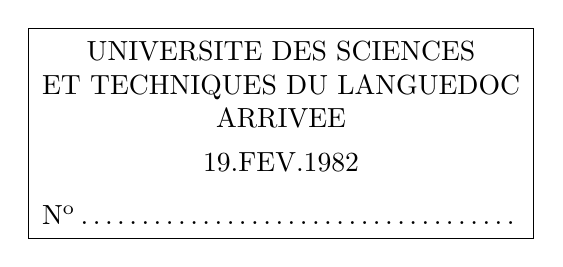
\begin{tikzpicture}\node[draw,align=center,inner sep=5pt] {\unsure{UNIVERSITE DES SCIENCES}\\\unsure{ET TECHNIQUES DU LANGUEDOC}\\\unsure{ARRIVEE}\\[4pt]19.FEV.1982\\[7pt]N\textsuperscript{o}\dotfill};\end{tikzpicture}}
\unsure{N\textsuperscript{o}}\quad 0153

\uline{OBJET} : Recrutement d'enseignants en coopération.

Le Ministère des Relations Extérieures vient de me faire tenir l'état des besoins en personnels enseignants dans les universités maghrébines pour l'année 1982 - 1983.

Je vous serais très obligé de bien vouloir procéder à la diffusion la plus large possible de cette liste dans votre établissement.

En effet, les premières sessions des Commissions Mixtes de recrutement pour les trois pays du Maghreb, doivent se tenir sous peu.

Il serait souhaitable d'inviter les candidats enseignants titulaires d'un grade de l'enseignement supérieur et les candidats non titulaires à adresser, directement et dans les meilleurs délais, leur demande accompagnée de leur curriculum vitae au C.F.E.C.T.I. \unsure{Carrefcur|Carrefour} coopération - 34, rue Dumont Durville 75016 PARIS.

En ce qui concerne les professeurs agrégés du second degré ou les titulaires de l'enseignement technique, ils devront transmettre d'urgence leur candidature et leur curriculum vitae au Ministère de l'Education Nationale - Direction des Personnels Enseignants de Lycées - Service de la réglementation et de la gestion - sous direction de la gestion des personnels enseignants - Bureau D P E 9 - 34, rue de Châteaudun - 75009 PARIS.

\figure{\begin{tikzpicture}\draw[thick] (0,0)--(8,0);\draw[thick] (7.65,.2)--(9.5,-2.8);\end{tikzpicture}}
DIFFUSION : LISTE C n\textsuperscript{o} 1049, NC.PB

Transmis par la Cellule des Relations Internationales (bâtiment administratif, niveau haut) où vous pourrez consulter la liste des postes par disciplines et grades

MONTPELLIER, le 23 Février 1982

Le Délégué aux Relations\par Internationales

\figure{
\begin{tikzpicture}[scale=.65]\draw (0,0)--(.45,1.4)--(.65,-.15) (.03,.3)--(.8,.7);\draw (.6,.1) .. controls (1.1,1.7) and (1.7,1.8) .. (.9,.5) .. controls (1.2,.5) and (1.4,1.4) .. (1.55,1.25) .. controls (1.3,.8) and (1.1,.2) .. (1.5,.4) .. controls (1.65,.8) and (1.65,1.05) .. (1.75,.4) .. controls (1.75,.2) and (1.95,.9) .. (2.1,.75) .. controls (2.4,.6) and (2.6,1.2) .. (2.8,.8) .. controls (3,.8) and (2.5,.1) .. (2.75,.2);\draw (0,-.1)--(3.6,1);\end{tikzpicture}}
A. PAVIA

L'Adjoint au Délégué\par chargé des Affaires Administratives\par et Financières

\figure{
\begin{tikzpicture}[scale=.7]\draw (0,.9)--(5,2.3) (0,.9) .. controls (1.1,.85) and (1.6,.85) .. (1.8,.5);\draw (1,.1)--(1.2,1.8) (1.15,.05) .. controls (1.65,2.9) and (2.1,3) .. (1.9,.5) .. controls (1.9,.1) and (2.2,.1) .. (2.15,1.45) .. controls (2.2,.1) and (2.5,.1) .. (2.5,1.7) .. controls (2.65,-.05) and (2.9,.2) .. (2.85,1.5) .. controls (2.9,.2) and (3.1,.45) .. (3.15,1.45) .. controls (3.3,.5) and (3.45,.85) .. (3.5,.9) .. controls (4,.2) and (4.35,.65) .. (4.45,1.6);\draw (4.5,2.15)--(4.65,-.15) (1.4,-.1)--(5.2,.9);\end{tikzpicture}}
Jean Louis DEVAUX
\mspage{45}
